% ============================================================
% Member 1: Validation Strategy and Physics Baseline
% Upload figures/baseline_predicted_vs_actual.png to the Overleaf
% figures folder before compiling.
% ============================================================

\section{Validation Strategy}

We split the cleaned and feature engineered Kaggle table (68,711 rows) into three parts: 70\% for training, 15\% for validation, and 15\% for testing. The split is done in two steps with \texttt{train\_test\_split} from Scikit-Learn and a fixed seed (\texttt{random\_state=42}): first 30\% of the rows are held out, and then that 30\% is cut in half into the validation and test sets. Using a fixed seed means every run, and every member's code, gets exactly the same rows in each set.

Each set has a clear job:

\begin{itemize}
    \item \textbf{Training set:} used to fit the models (and the single constant of the physics baseline).
    \item \textbf{Validation set:} used to compare hyperparameter settings and pick the final ones.
    \item \textbf{Test set:} kept aside until the very end and used once to report the final results, so the reported numbers are not influenced by tuning.
\end{itemize}

The script \texttt{src/split\_data.py} creates the split, checks that no row appears in more than one set, and confirms that it is identical to the split used by the models in \texttt{src/model.py}. This guarantees that the gradient boosting model, the neural network, and the physics baseline are all tested on exactly the same rows.

Table~\ref{tab:split} shows that the three sets look alike. The average DC power differs by less than 0.4\% between them, and the share of zero output rows (mostly night time and the edges of the day) is about 46\% in each. This means the test set is a fair sample of the data and none of the sets is easier or harder by chance.

\begin{table}[h]
\centering
\begin{tabular}{lrrrrr}
\hline
\textbf{Set} & \textbf{Rows} & \textbf{Share} & \textbf{Mean DC power} & \textbf{Std. dev.} & \textbf{Zero output} \\
\hline
Train      & 48,097 & 70.0\% & 3149.91 & 4039.76 & 46.4\% \\
Validation & 10,307 & 15.0\% & 3145.62 & 4035.85 & 46.6\% \\
Test       & 10,307 & 15.0\% & 3155.23 & 4026.74 & 46.2\% \\
\hline
\end{tabular}
\caption{Size and target statistics of the three sets (from \texttt{results/split\_summary.csv}).}
\label{tab:split}
\end{table}

We chose a single fixed split instead of K fold cross validation for two reasons. The dataset is large enough (over 10,000 rows in each of the validation and test sets) for one split to give stable results, and training the neural network many times for every hyperparameter setting would have taken much longer. The main weakness of a random split on 15 minute data is that neighbouring readings, which are very similar, can end up in different sets; this is discussed in the Limitations section.

\section{Physics Baseline}

To show whether machine learning actually adds value, we compare our models against the standard way solar output is estimated without ML. The baseline in \texttt{src/physics\_baseline.py} uses a fixed formula:

\begin{equation}
P = k \cdot G \cdot \bigl(1 + \gamma\,(T_{\text{module}} - 25)\bigr)
\end{equation}

where $P$ is the predicted DC power, $G$ is the irradiation, $T_{\text{module}}$ is the panel temperature in $^{\circ}$C, and $\gamma = -0.004$, a typical value for silicon panels. In words, output grows in proportion to sunlight and drops by about 0.4\% for every degree the panel is hotter than 25\,$^{\circ}$C. The constant $k$ represents the size of the plant. It is the only number the baseline learns, and it is fitted once on the training set by least squares. The baseline uses the original, unscaled sunlight and temperature values, and is evaluated on the same validation and test rows as the ML models with the same MAE, RMSE, and R$^2$ functions.

We also tested a simpler version that uses sunlight only, without the temperature correction, to see how much the temperature term helps. Table~\ref{tab:baseline} shows the test results next to the two ML models.

\begin{table}[h]
\centering
\begin{tabular}{lrrr}
\hline
\textbf{Model (test set)} & \textbf{MAE} & \textbf{RMSE} & \textbf{R$^2$} \\
\hline
Physics baseline (sunlight only)          & 234.89 & 503.25 & 0.9844 \\
Physics baseline (sunlight + temperature) & 208.32 & 466.90 & 0.9866 \\
Neural network                            & 178.26 & 417.49 & 0.9892 \\
Gradient boosting                         & 153.59 & 369.18 & 0.9916 \\
\hline
\end{tabular}
\caption{Physics baselines compared with the ML models on the test set.}
\label{tab:baseline}
\end{table}

\begin{figure}[h]
\centering
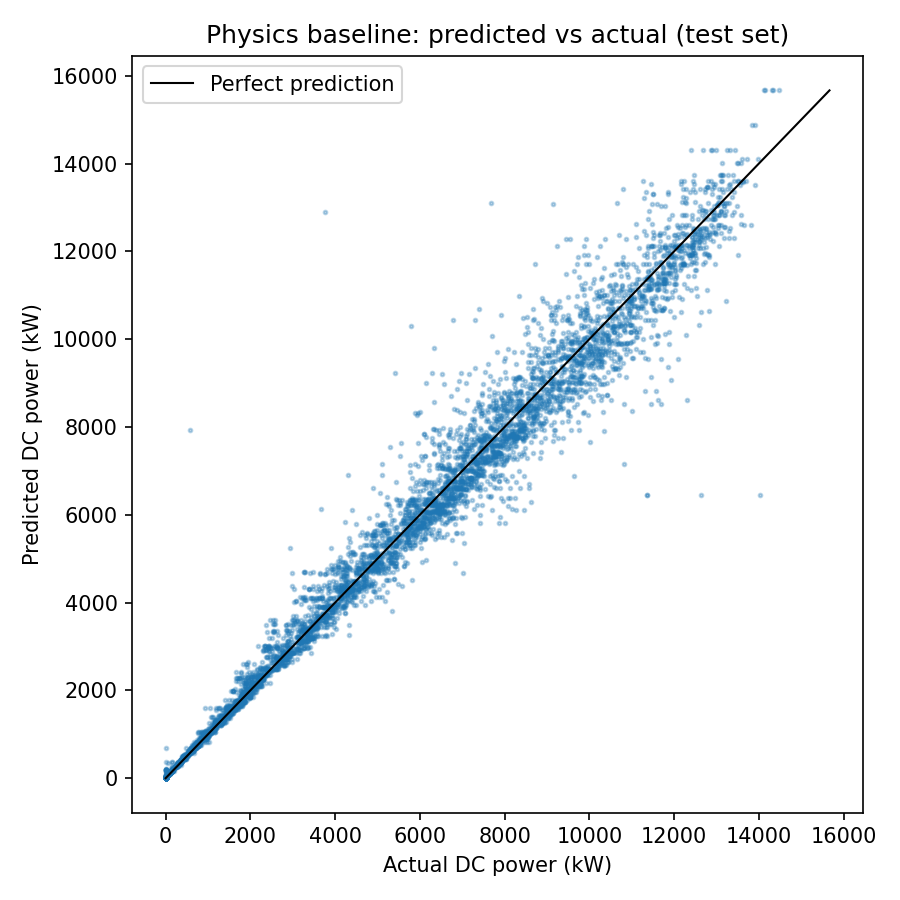
\includegraphics[width=0.6\textwidth]{baseline_predicted_vs_actual.png}
\caption{Predicted against actual DC power for the physics baseline (sunlight + temperature) on the test set.}
\label{fig:baseline}
\end{figure}

Three things stand out from these results:

\begin{itemize}
    \item \textbf{The baseline is already strong.} An R$^2$ of 0.987 matches what our exploratory analysis found: sunlight alone explains almost all of the change in output ($r = 0.993$). Any useful model has to beat this, which makes it an honest comparison.
    \item \textbf{The temperature correction helps.} Adding it lowers the MAE from 234.89 to 208.32 (about 11\%) and the RMSE by about 7\%, which confirms that hot panels really do produce less.
    \item \textbf{Machine learning still does clearly better.} Gradient boosting has about 26\% lower MAE and 21\% lower RMSE than the best baseline, and the neural network about 14\% lower MAE and 11\% lower RMSE. The ML models learn effects the formula cannot, such as differences between inverters and how output changes through the day.
\end{itemize}

For SunCast, this gap matters because errors in the power forecast carry straight into the savings estimate a user sees. The baseline will also be useful in the app as a fallback and as a sanity check on the model's predictions.